\documentclass[12pt, titlepage]{article}
\usepackage{float}
\usepackage{booktabs}
\usepackage{tabularx}
\usepackage{hyperref}
\usepackage{pgfplots}
\usepackage{comment}
\pgfplotsset{compat=1.18}
\usepackage[table]{xcolor}
\hypersetup{
    colorlinks,
    citecolor=black,
    filecolor=black,
    linkcolor=red,
    urlcolor=blue
}
\usepackage[round]{natbib}
\usepackage{graphicx}

\input{../Comments}
%% Common Parts

\newcommand{\progname}{Software Engineering} % PUT YOUR PROGRAM NAME HERE
\newcommand{\authname}{Team 8, AlgoCatan
\\ Jake Read
\\ Rebecca Di Filippo
\\ Matthew Cheung
\\ Sunny Yao} % AUTHOR NAMES

\usepackage{hyperref}
    \hypersetup{colorlinks=true, linkcolor=blue, citecolor=blue, filecolor=blue,
                urlcolor=blue, unicode=false}
    \urlstyle{same}
                                


\begin{document}

\title{Verification and Validation Report: \progname} 
\author{\authname}
\date{\today}
	
\maketitle

\pagenumbering{roman}

\section{Revision History}

\begin{tabularx}{\textwidth}{p{3cm}p{2cm}X}
\toprule {\bf Date} & {\bf Version} & {\bf Notes}\\
\midrule
March 4th & 1.0 & Draft from VNV plan\\
March 9th & 1.1 & Updated VNV report\\
April 6th 2026 & Final & Feedback from TA for final documentation\\
\bottomrule
\end{tabularx}

~\newpage

\section{Symbols, Abbreviations and Acronyms}

\renewcommand{\arraystretch}{1.2}
\begin{tabular}{l l} 
  \toprule		
  \textbf{symbol} & \textbf{description}\\
  \midrule 
  AI & Artifical Intelligence\\
  \bottomrule
\end{tabular}\\

\newpage

\tableofcontents

\listoftables %if appropriate

\listoffigures %if appropriate

\newpage

\pagenumbering{arabic}

\section{Functional Requirements Evaluation}

\section{System Tests}

This section details the system-level tests for validating the functional and non-functional requirements of the AlgoCatan system. These tests are designed to be run once the integrated system is complete, using representative data to simulate actual gameplay and training cycles.

\subsection{Tests for Functional Requirements}

The tests below are categorized by the major functional modules defined in Section S.2 of the SRS to ensure 100\% coverage.

\subsubsection{Computer Vision Model (S.2.1)}
\textit{Status: NOT IMPLEMENTED (Out of Scope / Deferred)}

\begin{enumerate}
    \item{\hypertarget{T.FR.CV.1.1}{T.FR.CV.1.1} (DEFERRED)\\}
    \textbf{Initial State:} Physical board setup with known assets.\\
    \textbf{Input:} Captured camera feed.\\
    \textbf{Output:} Structured data matching physical state with 99.99\% accuracy.\\
    \textbf{Derivation:} Verifies $\hyperref[FR.S.1.1]{FR.S.1.1}$, $\hyperref[FR.S.1.2]{FR.S.1.2}$, $\hyperref[FR.S.1.3]{FR.S.1.3}$, $\hyperref[FR.S.1.4]{FR.S.1.4}$, $\hyperref[FR.S.1.5]{FR.S.1.5}$.
\end{enumerate}

\subsubsection{Training Pipeline \& AI Model (S.2.2 \& S.2.3)}

\begin{enumerate}
    \item{\hypertarget{T.FR.AI.2.1}{T.FR.AI.2.1}\\}
    \textbf{Control:} Automatic \\
    \textbf{Initial State:} AI Model loaded into the Training Pipeline. \\
    \textbf{Input:} Trigger self-play training session using Elo League for opponent selection. \\
    \textbf{Output:} System executes moves following official Catan rules ($\hyperref[FR.S.2.1]{FR.S.2.1}$), generates success rewards ($\hyperref[FR.S.2.3]{FR.S.2.3}$), and saves model snapshots.\\
    \textbf{Derivation:} Verifies $\hyperref[FR.S.2.1]{FR.S.2.1}$, $\hyperref[FR.S.2.2]{FR.S.2.2}$, $\hyperref[FR.S.2.3]{FR.S.2.3}$, $\hyperref[FR.S.2.4]{FR.S.2.4}$, $\hyperref[FR.S.2.5]{FR.S.2.5}$, $\hyperref[FR.S.3.5]{FR.S.3.5}$.

    \item{\hypertarget{T.FR.AI.2.2}{T.FR.AI.2.2}\\}
    \textbf{Control:} Automatic \\
    \textbf{Initial State:} A GameState where only one legal move exists (e.g., specific road placement).\\
    \textbf{Input:} Process state through the AI Model. \\
    \textbf{Output:} AI returns the single valid action consistent with Catan rules. \\
    \textbf{Derivation:} Verifies $\hyperref[FR.S.3.1]{FR.S.3.1}$, $\hyperref[FR.S.3.2]{FR.S.3.2}$.

    \item{\hypertarget{T.FR.AI.2.3}{T.FR.AI.2.3}\\}
    \textbf{Control:} Automatic \\
    \textbf{Initial State:} 100 matches played against a "Random Move" bot. \\
    \textbf{Output:} The AI Model must achieve a win rate $>50\%$. \\
    \textbf{Derivation:} Verifies $\hyperref[FR.S.3.4]{FR.S.3.4}$.

    \item{\hypertarget{T.FR.AI.2.4}{T.FR.AI.2.4}\\}
    \textbf{Control:} Manual \\
    \textbf{Initial State:} UI is active and a game is in progress using "Model v1.0". \\
    \textbf{Input:} User uses the interface to select and load "Model v2.0" from the Elo League list mid-game. \\
    \textbf{Output:} The system switches models without state loss; subsequent advice is generated by the newly selected model. \\
    \textbf{Derivation:} Verifies $\hyperref[FR.S.3.3]{FR.S.3.3}$.
\end{enumerate}

\subsubsection{Elo League System (S.2.4)}
\begin{enumerate}
    \item{\hypertarget{T.FR.ELO.3.1}{T.FR.ELO.3.1}\\}
    \textbf{Control:} Automatic \\
    \textbf{Initial State:} League contains 125 model snapshots. Model A (1200 Elo) plays Model B (1000 Elo). \\
    \textbf{Input:} Model A wins the match. \\
    \textbf{Output:} Elo ratings update via standard formula ($\hyperref[FR.S.3.7]{FR.S.3.7}$). The oldest/weakest model is pruned to maintain the 125-cap ($\hyperref[FR.S.3.10]{FR.S.3.10}$). \\
    \textbf{Derivation:} Verifies $\hyperref[FR.S.3.6]{FR.S.3.6}$, $\hyperref[FR.S.3.7]{FR.S.3.7}$, $\hyperref[FR.S.3.8]{FR.S.3.8}$, $\hyperref[FR.S.3.9]{FR.S.3.9}$, $\hyperref[FR.S.3.10]{FR.S.3.10}$.
\end{enumerate}

\subsubsection{Curriculum Learning Manager (S.2.5)}
\begin{enumerate}
    \item{\hypertarget{T.FR.CURR.4.1}{T.FR.CURR.4.1}\\}
    \textbf{Control:} Automatic \\
    \textbf{Initial State:} Training in Phase 1 (5 VP target). Advancement threshold set to 60\% win rate. \\
    \textbf{Input:} Training metrics reach 61\% win rate over 50 episodes. \\
    \textbf{Output:} System logs transition and automatically advances to Phase 2 (10 VP target). \\
    \textbf{Derivation:} Verifies $\hyperref[FR.S.3.12]{FR.S.3.12}$, $\hyperref[FR.S.3.13]{FR.S.3.13}$, $\hyperref[FR.S.3.14]{FR.S.3.14}$, $\hyperref[FR.S.3.15]{FR.S.3.15}$, $\hyperref[FR.S.3.16]{FR.S.3.16}$.
\end{enumerate}

\subsubsection{User Interface (S.2.6)}
\begin{enumerate}
    \item{\hypertarget{T.FR.UI.5.1}{T.FR.UI.5.1}\\}
    \textbf{Control:} Manual \\
    \textbf{Initial State:} Web interface open on both desktop and mobile devices. \\
    \textbf{Input:} User selects an opponent from the Elo League list and performs a build action. \\
    \textbf{Output:} UI displays the board in real-time ($\hyperref[FR.S.4.1]{FR.S.4.1}$), reflects the build action immediately ($\hyperref[FR.S.4.2]{FR.S.4.2}$), and scales correctly to the mobile screen size ($\hyperref[FR.S.4.5]{FR.S.4.5}$). \\
    \textbf{Derivation:} Verifies $\hyperref[FR.S.4.1]{FR.S.4.1}$, $\hyperref[FR.S.4.2]{FR.S.4.2}$, $\hyperref[FR.S.4.3]{FR.S.4.3}$, $\hyperref[FR.S.4.5]{FR.S.4.5}$, $\hyperref[FR.S.4.7]{FR.S.4.7}$, $\hyperref[FR.S.4.8]{FR.S.4.8}$.
\end{enumerate}

\subsubsection{Game State Database \& Manager (S.2.7 \& S.2.9)}
\begin{enumerate}
\item{\hypertarget{T.FR.DATA.6.1}{T.FR.DATA.6.1}\\}
  \textbf{Control:} Automatic \\
  \textbf{Initial State:} Active game session in progress. \\
  \textbf{Input:} A player performs a "Build City" action; the system process is then forcibly terminated (simulated crash). \\
  \textbf{Output:} Upon system restart, the Game State Manager successfully recovers the session from the database. The board state accurately reflects the built City and updated resource inventories ($\hyperref[FR.S.5.4]{FR.S.5.4}$). \\
  \textbf{Derivation:} Verifies $\hyperref[FR.S.5.1]{FR.S.5.1}$, $\hyperref[FR.S.5.2]{FR.S.5.2}$, $\hyperref[FR.S.5.4]{FR.S.5.4}$, $\hyperref[FR.S.7.1]{FR.S.7.1}$, $\hyperref[FR.S.7.2]{FR.S.7.2}$, $\hyperref[FR.S.7.4]{FR.S.7.4}$, $\hyperref[FR.S.7.5]{FR.S.7.5}$.
\end{enumerate}

\begin{enumerate}
\item{\hypertarget{T.FR.DATA.6.2}{T.FR.DATA.6.2}\\}
\textbf{Control:} Automatic \\
\textbf{Initial State:} The Game State Database contains at least one record of a 50+ turn game. \\
\textbf{Input:} A request is sent via the API to retrieve the structured history (specifically dice rolls and turn transitions) for the session. \\
\textbf{Output:}\\
    a) The database returns the complete, timestamped log of all dice rolls and turn transitions without data loss ($\hyperref[FR.S.7.3]{FR.S.7.3}$).  \\
    b) The structured data is formatted for replay/analysis and returned within the efficiency targets for read operations ($\hyperref[FR.S.5.3]{FR.S.5.3}$, $\hyperref[FR.S.5.5]{FR.S.5.5}$). \\
\textbf{Derivation:} Verifies $\hyperref[FR.S.5.3]{FR.S.5.3}$, $\hyperref[FR.S.5.5]{FR.S.5.5}$, $\hyperref[FR.S.7.3]{FR.S.7.3}$.
\end{enumerate}

\subsubsection{Backend API Server (S.2.8)}

\begin{enumerate}
    \item{\hypertarget{T.FR.API.7.1}{T.FR.API.7.1}\\}
    \textbf{Control:} Automatic \\
    \textbf{Initial State:} System under normal load. \\
    \textbf{Input:} UI sends a move request to the AI via the API. \\
    \textbf{Output:} UI update latency is $<100ms$ and AI decision return is $<1s$. \\
    \textbf{Derivation:} Verifies $\hyperref[FR.S.6.1]{FR.S.6.1}$, $\hyperref[FR.S.6.2]{FR.S.6.2}$, $\hyperref[FR.S.6.3]{FR.S.6.3}$.
\end{enumerate}

\subsubsection{Explanation Pipeline (S.2.10)}

\begin{enumerate}
    \item{\hypertarget{T.FR.EXP.8.1}{T.FR.EXP.8.1}\\}
    \textbf{Control:} Manual \\
    \textbf{Initial State:} AI makes a move (e.g., placing a robber on a Wheat tile). \\
    \textbf{Input:} User clicks "Explain Move" in the UI. \\
    \textbf{Output:} The LLM generates a natural language response which is displayed in the UI.\\
    \textbf{Derivation:} Verifies $\hyperref[FR.S.4.4]{FR.S.4.4}$, $\hyperref[FR.S.4.6]{FR.S.4.6}$, $\hyperref[FR.S.8.1]{FR.S.8.1}$, $\hyperref[FR.S.8.2]{FR.S.8.2}$, $\hyperref[FR.S.8.3]{FR.S.8.3}$.
\end{enumerate}

\subsection{Traceability Between Test Cases and Requirements}

\begin{table}[H]
  \centering
  \caption{Functional Requirement Traceability Matrix}
  \label{tab:traceability}
  \begin{tabularx}{\textwidth}{|c|>{\raggedright\arraybackslash}X|}
    \hline
    \textbf{Test Case ID} & \textbf{Requirements Verified} \\
    \hline
    \hyperlink{T.FR.CV.1.1}{T.FR.CV.1.1} & FR.S.1.1, FR.S.1.2, FR.S.1.3, FR.S.1.4, FR.S.1.5 (DEFERRED) \\
    \hline
    \hyperlink{T.FR.AI.2.1}{T.FR.AI.2.1} & FR.S.2.1, FR.S.2.2, FR.S.2.3, FR.S.2.4, FR.S.2.5, FR.S.3.5 \\
    \hline
    \hyperlink{T.FR.AI.2.2}{T.FR.AI.2.2} & FR.S.3.1, FR.S.3.2 \\
    \hline
    \hyperlink{T.FR.AI.2.3}{T.FR.AI.2.3} & FR.S.3.4 \\
    \hline
    \hyperlink{T.FR.AI.2.4}{T.FR.AI.2.4} & FR.S.3.3 \\
    \hline
    \hyperlink{T.FR.ELO.3.1}{T.FR.ELO.3.1} & FR.S.3.6, FR.S.3.7, FR.S.3.8, FR.S.3.9, FR.S.3.10 \\
    \hline
    \hyperlink{T.FR.CURR.4.1}{T.FR.CURR.4.1} & FR.S.3.12, FR.S.3.13, FR.S.3.14, FR.S.3.15, FR.S.3.16 \\
    \hline
    \hyperlink{T.FR.UI.5.1}{T.FR.UI.5.1} & FR.S.4.1, FR.S.4.2, FR.S.4.3, FR.S.4.5, FR.S.4.7, FR.S.4.8 \\
    \hline
    \hyperlink{T.FR.DATA.6.1}{T.FR.DATA.6.1} & FR.S.5.1, FR.S.5.2, FR.S.5.4, FR.S.7.1, FR.S.7.2, FR.S.7.4, FR.S.7.5 \\
    \hline
    \hyperlink{T.FR.DATA.6.2}{T.FR.DATA.6.2} & FR.S.5.3, FR.S.5.5, FR.S.7.3 \\
    \hline
    \hyperlink{T.FR.API.7.1}{T.FR.API.7.1} & FR.S.6.1, FR.S.6.2, FR.S.6.3 \\
    \hline
    \hyperlink{T.FR.EXP.8.1}{T.FR.EXP.8.1} & FR.S.4.4, FR.S.4.6, FR.S.8.1, FR.S.8.2, FR.S.8.3 \\
    \hline
  \end{tabularx}
\end{table}


\section{Nonfunctional Requirements Evaluation}

\section{Tests for Nonfunctional Requirements}

This section outlines the system-level tests for validating the nonfunctional requirements (NFRs) defined in Section~S.2.8 of the SRS. These include scalability, usability, maintainability, installability, data integrity, and availability.

Each subsection corresponds to a major nonfunctional quality attribute of the AlgoCatan system. Some tests produce summary statistics or qualitative evaluations (e.g., graphs or surveys) rather than strict pass/fail outcomes.

Accuracy-related nonfunctional qualities are validated implicitly through the functional tests defined in Section~4.2 (T.FR.AI.2.1--2.3 and T.FR.CV.1.1--1.2), which record relative error and correctness metrics.

\subsection{Performance and Scalability}

This area ensures acceptable responsiveness and throughput under varying load.

\textbf{Test Case: Baseline Performance}

\begin{enumerate}
\item{\hypertarget{T.NFR.P.1}{T.NFR.P.1}\\}
\textbf{Control:} Automatic

\textbf{Initial State:} AlgoCatan server running full stack with no concurrent load.

\textbf{Input/Condition:} Single 4-player game with standard actions (build, trade, roll dice, 100+ repetitions).

\textbf{Performance Thresholds:}
\begin{itemize}
    \item AI Move Suggestion: $\leq 500$ms avg, $\leq 750$ms peak
    \item Board State Update: $\leq 200$ms avg, $\leq 300$ms peak
    \item UI Render: $\leq 50$ms/frame
\end{itemize}

\textbf{How tested:} Automated with server-side logging and Chrome DevTools Performance API.

\textbf{Trace:} NFR.S.1
\end{enumerate}

\textbf{Test Case: Scalability Under Load}

\begin{enumerate}
\item{\hypertarget{T.NFR.P.2}{T.NFR.P.2}\\}
\textbf{Control:} Automatic

\textbf{Initial State:} AlgoCatan server running full stack.

\textbf{Input/Condition:} Simulate 1, 3, and 5 concurrent games.
Measure response time scaling.

\textbf{Scalability Thresholds (Sub-Linear Growth):}
\begin{itemize}
    \item Response time at 3 games $\leq 1.5 \times$ single game
    \item Response time at 5 games $\leq 2.0 \times$ single game
    \item CPU utilization $\leq 80\%$ at 5 games
    \item No memory leaks or OOM errors over 1+ hour
\end{itemize}

\textbf{How tested:} Automated load-testing scripts with system monitoring.
Pass if all thresholds met.

\textbf{Trace:} NFR.S.1
\end{enumerate}

\subsection{Usability}

This area focuses on confirming that the interface is intuitive and accessible to users with minimal training. It also includes accessibility checks for users with visual impairments.

\textbf{Test Case: Usability Survey and User Feedback}

\begin{enumerate}
\item{\hypertarget{T.NFR.U.1}{T.NFR.U.1}\\}
\textbf{Control:} Manual

\textbf{Initial State:} Final prototype deployed in a browser.

\textbf{Input/Condition:} 5-10 participants familiar with Catan complete a observational study and fill out the usability survey (Appendix 7.2).

\textbf{Output/Result:} Average rating $\geq 4/5$ for clarity, ease of navigation, and intuition.

\textbf{Test Case Derivation:} Verifies NFR.S.2 (Usability) through direct user evaluation.

\textbf{How test will be performed:} Conducted during the final demo; results aggregated and visualized as a bar chart.
\end{enumerate}

\textbf{Test Case: Accessibility and Visual Clarity}

\begin{enumerate}
\item{\hypertarget{T.NFR.U.2}{T.NFR.U.2}\\}
\textbf{Control:} Manual

\textbf{Initial State:} AlgoCatan UI loaded in browser.

\textbf{Input/Condition:} Apply color-blindness filters and vary display scaling.

\textbf{Output/Result:} All critical UI elements remain legible; contrast ratio $\geq 4.5:1$.

\textbf{Test Case Derivation:} Verifies accessibility and clarity under varied visual conditions.

\textbf{How test will be performed:} Tested using Chrome DevTools accessibility simulator; screenshots recorded for documentation.
\end{enumerate}

\subsection{Maintainability}

This area ensures the modular design and structure of the codebase support efficient updates and debugging.

\textbf{Test Case: Code Quality and Modular Design Inspection}

\begin{enumerate}
\item{\hypertarget{T.NFR.M.1}{T.NFR.M.1}\\}
\textbf{Control:} Static

\textbf{Initial State:} Complete source code committed to GitHub.

\textbf{Input/Condition:} Run \texttt{SonarQube} and \texttt{flake8} to generate maintainability and style reports.

\textbf{Output/Result:} No high-severity issues; modules follow consistent structure and clear separation of concerns.

\textbf{Test Case Derivation:} Verifies NFR.S.3 (Maintainability) through code inspection and static analysis.

\textbf{How test will be performed:} Peer inspection led by group members; issues logged in GitHub for resolution.
\end{enumerate}

\subsection{Installability}

This area validates that AlgoCatan installs and operates correctly across all supported operating systems and browsers.

\textbf{Test Case: Cross-Platform Installation Validation}

\begin{enumerate}
\item{\hypertarget{T.NFR.I.1}{T.NFR.I.1}\\}
\textbf{Control:} Manual

\textbf{Initial State:} Packaged release available.

\textbf{Input/Condition:} Install and execute AlgoCatan on Windows~11 and macOS using Chrome and Firefox browsers.

\textbf{Output/Result:} Application installs and runs successfully on all tested platforms.

\textbf{Test Case Derivation:} Verifies NFR.S.4 (Installability) by ensuring cross-platform compatibility.

\textbf{How test will be performed:} Each team member installs on a unique OS following a checklist; issues recorded and documented.
\end{enumerate}

\subsection{Data Integrity}

This area ensures that the Game State Database maintains consistent, valid, and accurate data under all conditions, including normal operation, concurrent updates, and unexpected failures. This includes validation of incoming updates and transactional consistency to prevent corruption.

\textbf{Test Case: Transaction Integrity and Recovery}

\begin{enumerate}
\item{\hypertarget{T.NFR.D.1}{T.NFR.D.1}\\}
\textbf{Control:} Automatic

\textbf{Initial State:} Active game session connected to the database.

\textbf{Input/Condition:} Execute 10 consecutive state updates with an artificial network interruption during one update.

\textbf{Output/Result:} Database remains consistent; interrupted transaction is rolled back cleanly; no other game states are affected.

\textbf{Test Case Derivation:} Verifies transactional consistency portion of NFR.S.5 under failure conditions.

\textbf{How test will be performed:} Automated integration test simulates network failures and verifies database consistency after each run.
\end{enumerate}

\textbf{Test Case: Data Validation on Updates}

\begin{enumerate}
\item{\hypertarget{T.NFR.D.2}{T.NFR.D.2}\\}
\textbf{Control:} Automatic

\textbf{Initial State:} Active game session connected to the database.

\textbf{Input/Condition:} Attempt to submit invalid game state updates, such as negative resource counts, illegal moves, or missing required fields.

\textbf{Output/Result:} Invalid updates are recognized and rejected.

\textbf{Test Case Derivation:} Verifies validation portion of NFR.S.5, preventing data corruption from malformed inputs.

\textbf{How test will be performed:} Automated tests inject invalid game state objects and verifies rejection.
\end{enumerate}

\textbf{Test Case: Concurrent Update Handling}

\begin{enumerate}
\item{\hypertarget{T.NFR.D.3}{T.NFR.D.3}\\}
\textbf{Control:} Automatic

\textbf{Initial State:} Two or more simultaneous game sessions active.

\textbf{Input/Condition:} Simulate concurrent updates to overlapping resources (e.g., two players updating the same tile).

\textbf{Output/Result:} Only one valid transaction is committed; conflicts are detected and resolved; no data corruption occurs.

\textbf{Test Case Derivation:} Verifies database integrity under concurrent operations, completing NFR.S.5 coverage.

\textbf{How test will be performed:} Automated integration tests run multiple simulated clients updating shared resources; system logs and database state are verified for correctness.
\end{enumerate}
\subsection{Availability}

This area verifies that the system maintains acceptable availability during use,
consistent with the SRS requirement that the system have an uptime of at least 99\%.

\textbf{Test Case: Service Availability Monitoring}

\begin{enumerate}
\item{\hypertarget{T.NFR.AV.1}{T.NFR.AV.1}\\}
\textbf{Control:} Automatic

\textbf{Initial State:} System deployed and running under normal usage conditions.

\textbf{Input/Condition:} Monitor backend service availability over the test period,
including normal gameplay, replay access, and explanation requests.

\textbf{Output/Result:} The backend API remains available for at least 99\% of the
observed test period.

\textbf{Test Case Derivation:} Verifies NFR.S.6 (Availability).

\textbf{How test will be performed:} Use uptime logs, health checks, and request
success/failure counts during the evaluation period to compute observed service availability.
\end{enumerate}

\subsection{Accuracy and Correctness (Referenced)}

Accuracy-related NFRs are verified by functional tests defined in Section~4.2:
\begin{itemize}
    \item T.FR.AI.2.1--2.3 (AI Model and Recommendation Logic)
    \item T.FR.CV.1.1 (Computer Vision and Game State Capture)
\end{itemize}
These tests report relative error between predicted and expected outcomes. No separate nonfunctional test cases are required.

\subsection{Traceability Between Test Cases and Requirements }

This subsection is limited to non-functional requirement traceability; the functional requirement traceability matrix is presented earlier in the Functional Requirements tests section.

\begin{table}[H]
  \centering
  \caption{Non-Functional Requirement Test Case Traceability Matrix}
  \label{tab:nfr-system-test-traceability}
  \begin{tabularx}{\textwidth}{|l|X|}
    \hline
    \textbf{Test Case ID} & \textbf{Requirement(s) Verified} \\ \hline
    \hyperlink{T.NFR.P.1}{T.NFR.P.1}   & NFR.S.1 -- Performance Baseline \\ \hline
    \hyperlink{T.NFR.P.2}{T.NFR.P.2}   & NFR.S.1 -- Scalability Under Load \\ \hline % Added missing ID
    \hyperlink{T.NFR.U.1}{T.NFR.U.1}   & NFR.S.2 -- Usability Survey \\ \hline
    \hyperlink{T.NFR.U.2}{T.NFR.U.2}   & NFR.S.2 -- Accessibility \\ \hline
    \hyperlink{T.NFR.M.1}{T.NFR.M.1}   & NFR.S.3 -- Maintainability \\ \hline
    \hyperlink{T.NFR.I.1}{T.NFR.I.1}   & NFR.S.4 -- Installability \\ \hline
    \hyperlink{T.NFR.D.1}{T.NFR.D.1}   & NFR.S.5 -- Transaction Consistency \\ \hline
    \hyperlink{T.NFR.D.2}{T.NFR.D.2}   & NFR.S.5 -- Data Validation \\ \hline
    \hyperlink{T.NFR.D.3}{T.NFR.D.3}   & NFR.S.5 -- Concurrency Handling \\ \hline
    \hyperlink{T.NFR.AV.1}{T.NFR.AV.1}  & NFR.S.6 -- Availability (Recovery \& Uptime) \\ \hline
  \end{tabularx}
\end{table}

\section{Unit Testing}

\subsection{Overview and Integration with System Tests}

This section documents the unit testing activities performed to verify individual components and modules of the RLCatan system at the code level. These unit tests complement the system-level tests described in Section~3 (Functional Requirements Evaluation) by providing detailed verification of API endpoints, utility functions, and integration points.

The unit tests are organized by functional module and include both dynamic testing (automated tests) and static analysis. These tests were executed as part of the continuous integration pipeline using Python's unittest/pytest framework for backend tests and integration with the API server for endpoint testing.

\subsection{Unit Testing Scope and Strategy}

\subsubsection{Scope}

The unit testing scope covers the following components:
\begin{itemize}
    \item Backend API endpoints and request/response handling
    \item Game State Manager and game creation/initialization
    \item Path resolution utilities for model asset loading
    \item Game analysis module integration with Monte Carlo Tree Search (MCTS) engine
    \item Database constraint validation and state management
\end{itemize}

Out of scope for unit testing:
\begin{itemize}
    \item External library verification (e.g., Catanatron, OpenAI Gym)
    \item React frontend component testing (addressed through usability testing in Section~3)
    \item LLM explanation pipeline (addressed through manual testing in Section~3)
    \item Computer Vision module (deferred and not implemented)
\end{itemize}

\subsubsection{Testing Strategy}

The unit testing strategy employs both white-box and black-box approaches:
\begin{itemize}
    \item \textbf{Black-box testing:} API endpoints are tested by sending HTTP requests and validating response structures and status codes without knowledge of internal implementation.
    \item \textbf{White-box testing:} Path resolution and game state validation functions are tested with knowledge of implementation to verify edge cases and internal state transitions.
    \item \textbf{Mocking and Isolation:} External dependencies (e.g., GameAnalyzer, database) are mocked to isolate units under test and verify behavior in controlled conditions.
\end{itemize}

\subsection{API and Game Management Module}

This module tests the backend API endpoints and game creation/initialization logic, supporting the system-level tests T.FR.AI.2.1, T.FR.API.7.1, and T.FR.DATA.6.1.

\begin{enumerate}

\item \texttt{test\_get\_bots\_endpoint}

\textbf{Type:} Functional, Dynamic, Automatic

\textbf{Initial State:} The API server is initialized and ready to receive requests.

\textbf{Input:} HTTP GET request to \texttt{/api/bots} endpoint.

\textbf{Expected Output:} 200 OK status code and JSON response containing list of available bot objects with at least 10 bots (including standard bots like \texttt{catanatron\_ab\_2}, \texttt{random}, \texttt{human}).

\textbf{Actual Output:} API returned 200 OK with complete bot registry containing 15 available bot configurations.

\textbf{Result:} Pass

\textbf{Requirement Traceability:} Supports FR.S.3.8 (exposing league members to UI), FR.S.4.7 (loading bot list), FR.S.4.8 (selecting opponents)

\textbf{Module Tested:} Backend API Server, Elo League System


\item \texttt{test\_stress\_test\_endpoint}

\textbf{Type:} Functional, Dynamic, Automatic

\textbf{Initial State:} The API server is initialized.

\textbf{Input:} HTTP GET request to \texttt{/api/stress-test} endpoint.

\textbf{Expected Output:} 200 OK status code and JSON object representing game state with essential structures: ``nodes'' and ``edges''.

\textbf{Actual Output:} Endpoint returned 200 OK with complete game state structure including board nodes and edges.

\textbf{Result:} Pass

\textbf{Requirement Traceability:} Supports FR.S.5.1 (storing complete game records), FR.S.7.5 (structured board access)

\textbf{Module Tested:} Backend API Server, Game State Manager


\item \texttt{test\_player\_factory\_custom\_bot}

\textbf{Type:} Functional, Dynamic, Automatic

\textbf{Initial State:} Internal functions mocked to simulate custom bot ``my\_custom\_bot''.

\textbf{Input:} POST request to \texttt{/api/games} with ``BOT:my\_custom\_bot'' in player list.

\textbf{Expected Output:} 200 OK response containing valid \texttt{game\_id}.

\textbf{Actual Output:} System correctly parsed custom bot prefix, retrieved mocked configuration, instantiated PPOPlayer with correct model path, and returned valid game ID.

\textbf{Result:} Pass

\textbf{Requirement Traceability:} Supports FR.S.2.5 (curriculum-guided RL with dynamic opponent selection), FR.S.3.3 (model versioning and interchange)

\textbf{Module Tested:} Backend API Server, Training Pipeline, AI Model integration


\item \texttt{test\_create\_game\_all\_player\_types}

\textbf{Type:} Functional, Dynamic, Automatic

\textbf{Initial State:} The API server is initialized.

\textbf{Input:} Series of POST requests to \texttt{/api/games} with different player types (CATANATRON, VALUE\_FUNCTION, HUMAN, PPO models).

\textbf{Expected Output:} 200 OK status code and valid \texttt{game\_id} for each request type.

\textbf{Actual Output:} All player type configurations successfully initialized; 5 game instances created with distinct player types all returned valid game IDs.

\textbf{Result:} Pass

\textbf{Requirement Traceability:} Supports FR.S.2.1 (rule enforcement in training), FR.S.2.2 (self-play with league opponents), FR.S.3.1 (valid game state analysis)

\textbf{Module Tested:} Backend API Server, Game State Manager, Training Pipeline

\end{enumerate}

\subsection{Path Resolution Module}

This module tests utility functions for safely resolving model asset paths across different deployment environments (HPC, local development, production).

\begin{enumerate}

\item \texttt{test\_resolve\_model\_path\_absolute\_hpc}

\textbf{Type:} Functional, Dynamic, Automatic

\textbf{Initial State:} Path resolution utilities loaded.

\textbf{Input:} Absolute file path string typical of HPC environment: \texttt{/nfs/features/rlcatan/models/v1.0}.

\textbf{Expected Output:} Normalized path rebased to local application directory structure: \texttt{/app/models/v1.0}.

\textbf{Actual Output:} Function correctly remapped HPC absolute path to application-local path structure.

\textbf{Result:} Pass

\textbf{Requirement Traceability:} Supports FR.S.2.2 (self-play training with correct model loading), FR.S.3.3 (seamless model interface)

\textbf{Module Tested:} AI Model, Training Pipeline (path resolution utility)


\item \texttt{test\_resolve\_model\_path\_relative}

\textbf{Type:} Functional, Dynamic, Automatic

\textbf{Initial State:} Path resolution utilities loaded.

\textbf{Input:} Standard relative path string: \texttt{data/models/v2}.

\textbf{Expected Output:} Absolute path correctly appending input to application root: \texttt{/app/data/models/v2}.

\textbf{Actual Output:} Function correctly resolved relative path to absolute application path.

\textbf{Result:} Pass

\textbf{Requirement Traceability:} Supports FR.S.2.2 (opponent selection and model loading in training), FR.S.3.3 (model versioning)

\textbf{Module Tested:} AI Model, Elo League System (model lookup and loading)

\end{enumerate}

\subsection{Game Analysis Module}

This module verifies integration with the Monte Carlo Tree Search (MCTS) engine for analyzing active games.

\begin{enumerate}

\item \texttt{test\_mcts\_analysis\_endpoint}

\textbf{Type:} Functional, Dynamic, Automatic

\textbf{Initial State:} Valid game created via API; GameAnalyzer mocked to return fixed win probabilities (e.g., RED=0.5, BLUE=0.3, WHITE=0.15, ORANGE=0.05).

\textbf{Input:} GET request to game's analysis URL: \texttt{/api/games/{game\_id}/mcts-analysis}.

\textbf{Expected Output:} 200 OK status and JSON response with \texttt{success=True} and win probabilities matching mocked values.

\textbf{Actual Output:} Endpoint correctly interfaced with mocked GameAnalyzer and returned expected win probability distribution.

\textbf{Result:} Pass

\textbf{Requirement Traceability:} Supports FR.S.3.4 (demonstrating AI learning through win probability analysis), FR.S.2.4 (batch and real-time evaluation modes)

\textbf{Module Tested:} Backend API Server, Game State Manager, Game Analysis integration


\item \texttt{test\_mcts\_analysis\_endpoint\_not\_found}

\textbf{Type:} Functional, Dynamic, Automatic

\textbf{Initial State:} The API server is initialized.

\textbf{Input:} GET request to analysis endpoint with non-existent game ID: \texttt{/api/games/99999/mcts-analysis}.

\textbf{Expected Output:} Error status code (404 Not Found or 500 Internal Server Error) without returning false success.

\textbf{Actual Output:} Endpoint correctly returned 404 Not Found with appropriate error message.

\textbf{Result:} Pass

\textbf{Requirement Traceability:} Supports robust error handling for FR.S.7.5 (structured game state access)

\textbf{Module Tested:} Backend API Server (error handling)

\end{enumerate}

\subsection{Database Constraint Validation Tests}

The following tests were executed as part of system-level test T.NFR.D-3 (Data Integrity - Concurrent Update Handling) and verify that the database layer enforces game state and action validity at the unit level.

\begin{enumerate}

\item \texttt{test\_invalid\_game\_state\_rejection}

\textbf{Type:} Functional, Dynamic, Automatic

\textbf{Initial State:} Database with transaction logging enabled.

\textbf{Input/Condition:} Attempt to store 15 intentionally invalid game states:
\begin{itemize}
    \item Negative resource counts
    \item Invalid player counts (0 or >4)
    \item Out-of-bounds settlement locations
    \item Impossible board configurations
\end{itemize}

\textbf{Expected Output:} 100\% rejection of invalid states; no invalid data persists in database.

\textbf{Actual Output:} All 15 invalid state payloads rejected by database constraint enforcement; verification queries confirmed no corrupted entries.

\textbf{Result:} Pass (15/15 test cases passed)

\textbf{Requirement Traceability:} Supports NFR.S.5 (Data Integrity - validation), FR.S.7.2 (accurate asset tracking)

\textbf{Module Tested:} Game State Database, Game State Manager


\item \texttt{test\_invalid\_action\_rejection}

\textbf{Type:} Functional, Dynamic, Automatic

\textbf{Initial State:} Active game session with action logging.

\textbf{Input/Condition:} Attempt to store 12 intentionally invalid actions:
\begin{itemize}
    \item Malformed move objects (missing required fields)
    \item References to non-existent game IDs
    \item Illegal moves (building where not allowed)
    \item Out-of-range action types
\end{itemize}

\textbf{Expected Output:} 100\% rejection of invalid actions; constraint violations logged.

\textbf{Actual Output:} All 12 invalid action payloads rejected at validation layer; violations correctly logged with detailed error messages.

\textbf{Result:} Pass (12/12 test cases passed)

\textbf{Requirement Traceability:} Supports FR.S.7.1 (rule-consistent state updates), FR.S.7.4 (automatic board state reflection)

\textbf{Module Tested:} Game State Database, Backend API Server (input validation)

\end{enumerate}

\subsection{Unit Test Summary and Coverage}

All unit tests executed successfully with 100\% pass rate across API endpoints, path resolution utilities, MCTS integration, and database constraint validation. These tests provide fine-grained verification that supports and complements the system-level tests documented in Section~3.

\subsubsection{Test Execution Coverage}

\begin{table}[H]
\centering
\begin{tabular}{|l|c|c|c|}
\hline
\textbf{Module} & \textbf{Unit Tests} & \textbf{Passed} & \textbf{Coverage} \\ \hline
API and Game Management & 4 & 4 & 100\% \\ \hline
Path Resolution & 2 & 2 & 100\% \\ \hline
Game Analysis (MCTS) & 2 & 2 & 100\% \\ \hline
Database Constraints & 2 & 2 & 100\% \\ \hline
\textbf{Total} & \textbf{10} & \textbf{10} & \textbf{100\%} \\ \hline
\end{tabular}
\caption{Unit Test Execution Summary}
\label{tab:unit-test-summary}
\end{table}



\section{Changes Due to Testing}

Based on testing results, we have identified and prioritized changes as follows:

\subsection*{High Priority (Rev 1 Implementation)}

\textbf{Change 1: UI Color-Coding and Visual Representation}

\textit{Test Evidence:} NFR.U.1 (Usability Survey) - 5 out of 7 participants (71\%) reported difficulty matching digital piece colors to physical Catan board expectations.
Catan-to-Bot Intuition score: 2.8/5.

\textit{What Changed:} Redesigned player color palette and piece representation to exactly match physical Catan board colors (Red=\#FF0000, Blue=\#0000FF, White=\#FFFFFF, Orange=\#FFA500).
Added resource token icons with color-blind-safe palettes and clear hexagon type labels.

\textit{Why:} Participants struggled with the digital-to-physical mapping, indicating a gap in FR.S.4.1 (Interactive Board View) and FR.S.4.2 (Visual Indicators) implementation.

\textit{Requirement Impact:} Directly improves FR.S.4.1, FR.S.4.2, and NFR.S.2 (Usability).
Expected post-implementation Intuition score: 4/5.

\textbf{Change 2: Game Flow Navigation Enhancement}

\textit{Test Evidence:} NFR.U.1 and NFR.U.2 (Usability/Accessibility) - 4 out of 7 participants requested clearer hexagon type labels.
Accessibility test showed text clarity issues at 80\% browser zoom.

\textit{What Changed:} Implemented permanent resource type labels on all hexagons (Wheat, Sheep, Brick, Ore, Lumber, Desert).
Created tooltip system with minimum 14pt font, scalable to 120\% with browser zoom.
Added visual action flow highlighting.

\textit{Why:} Unlabeled hexagons created cognitive load for new players, and accessibility failures could exclude users.
This directly addresses FR.S.4.3 (Action Controls) and FR.S.4.5 (Multi-Platform Support) gaps.

\textit{Requirement Impact:} Improves FR.S.4.3, FR.S.4.5, and NFR.S.2 (Usability/Accessibility).

\textbf{Change 3: Data Validation Layer Hardening}

\textit{Test Evidence:} T.NFR.D.1, T.NFR.D.2, T.NFR.D.3 (Data Integrity Tests) - All 15 invalid state payloads rejected (100\% success), all 12 invalid action payloads rejected (100\% success).

\textit{What Changed:} Added pre-storage validation checks for game state constraints.
Implemented comprehensive error logging with specific violation details.
Added database schema constraints (foreign keys, check constraints) as secondary protection layer.

\textit{Why:} Tests confirmed database integrity was working, but to prevent future regressions and improve auditability, we hardened the validation layer.

\textit{Requirement Impact:} Ensures FR.S.7.1 (Following Rules), FR.S.7.2 (Player Asset Tracking), and NFR.S.5 (Data Integrity) remain robust.
Prevents data corruption from persisting.

\subsection*{Medium Priority (Post-Rev 1 / Backlog)}

\textbf{Change 4: Performance Optimization}

\textit{Test Evidence:} T.NFR.P.1 and T.NFR.P.2 (Performance/Scalability) - AI Suggestion latency averaged 350ms (under 500ms target), Board Update averaged 85ms (under 200ms target), but UI render time averaged 45ms per frame (target 60fps = 16.67ms not achieved).

\textit{What Changed:} Optimized WebSocket message batching, implemented React memoization, migrated to canvas-based rendering for board, added server-side caching for state queries.

\textit{Why:} While meeting latency targets, frame rate indicated room for improvement to enhance perceived responsiveness.

\textit{Requirement Impact:} Improves NFR.S.1 (Scalability).
Target: 60fps (currently ~22fps post-optimization, further improvements deferred).

\textbf{Change 5: Unit Testing Framework Establishment}

\textit{Test Evidence:} 10 unit tests executed (100\% pass rate) covering API endpoints, path resolution, MCTS integration, database constraints.

\textit{What Changed:} Integrated pytest framework for all Python backend modules.
Added unit test execution to CI/CD pipeline (blocks merges on failure). Established 80\% minimum code coverage threshold for new contributions.
Created test documentation and examples.

\textit{Why:} Tests demonstrated modules work correctly in isolation, but formalizing the framework prevents future regressions.

\textit{Requirement Impact:} Improves NFR.S.3 (Maintainability).
Provides executable documentation for future developers.

\subsection*{Out of Scope}
The following findings from testing will not be addressed due to time constraints or project priorities:
\begin{itemize}
    \item \textbf{Low-Impact Security Issues:} SonarQube identified low-risk security issues.
    Given deployment context, these are deferred to future cycles.
    \item \textbf{Advanced Model Optimizations:} Testing revealed user experience is a larger bottleneck than AI model performance.
    Model optimization deferred in favor of usability improvements.
    \item \textbf{Deployment Strategy:} Currently using paid Render hosting.
    Long-term hosting decisions deferred post-project completion.
\end{itemize}

\subsection*{Summary}

Testing conclusions have shifted our priorities from improving the model's decision-making to enhancing the user experience and code quality.
The VnV process identified 5 concrete changes—3 implemented (UI/UX, data validation), 2 deferred (performance, testing framework)—demonstrating clear linkage between test results and quality improvements.
This evidence-based approach strengthens our confidence that the system meets both functional (FR.S.4.1-4.5, FR.S.7.1-7.2) and nonfunctional (NFR.S.2, NFR.S.5) requirements.

\section{Automated Testing}

For our functional and non-functional requirements evaluation, we employed bash scripts for specific testing purposes:
\begin{itemize}
    \item \textbf{Load/Stress Testing:} Bash scripts were used to send repeated requests to the API endpoints to measure response times and identify performance bottlenecks under load (satisfying NFR.E.4 and FR.S.6.3).
    \item \textbf{Game Simulation Testing:} Scripts automated the execution of multiple game scenarios to validate that the AI model produces legal moves and handles edge cases correctly (satisfying FR.S.3.1 and FR.S.3.2).
    \item \textbf{Integration Testing:} Bash scripts coordinated calls between modules to verify data flow and state consistency across the system (supporting FR.S.7 game state database requirements).
\end{itemize}

However, comprehensive unit testing with pytest and Jest was not fully implemented during this revision due to time constraints and the team's focus on system-level validation and usability testing.
The CI/CD pipeline was expanded to incorporate the bash scripts and static analysis tools, ensuring code stability and catching issues early in the development cycle.
The automated testing process includes running integration tests, linting, and coverage reporting through the GitHub Actions pipeline.

\section{Comprehensive Trace to Requirements}

This section provides detailed traceability between executed tests and requirements from the Software Requirements Specification (SRS), demonstrating complete coverage of the VnV Plan and consistency between planned and executed testing activities.

\subsection{Functional Requirements Trace - Detailed Coverage Analysis}

The following table maps each executed functional test to the specific requirements it verifies, organized by requirement ID. This addresses the professor's feedback regarding consistency between planned tests and requirements coverage.

\begin{table}[H]
\centering
\resizebox{\textwidth}{!}{%
\begin{tabular}{|c|c|c|c|}
\hline
\textbf{Requirement ID} & \textbf{Requirement Name} & \textbf{Test Case(s)} & \textbf{Status} \\ \hline
\hyperref[FR.S.1.1]{FR.S.1.1} & Visual Input Processing & T.FR.CV.1.1 & DEFERRED \\ \hline
\hyperref[FR.S.1.2]{FR.S.1.2} & Feature-to-State Translation & T.FR.CV.1.1 & DEFERRED \\ \hline
\hyperref[FR.S.1.3]{FR.S.1.3} & Error Detection and Correction & T.FR.CV.1.1 & DEFERRED \\ \hline
\hyperref[FR.S.1.4]{FR.S.1.4} & Dynamic Calibration & T.FR.CV.1.1 & DEFERRED \\ \hline
\hyperref[FR.S.1.5]{FR.S.1.5} & Diagnostic Feedback & T.FR.CV.1.1 & DEFERRED \\ \hline
\hyperref[FR.S.2.1]{FR.S.2.1} & Rule Simulation & T.FR.AI.2.1, unit tests & PASS \\ \hline
\hyperref[FR.S.2.2]{FR.S.2.2} & AI Training Integration & T.FR.AI.2.1, unit tests & PASS \\ \hline
\hyperref[FR.S.2.3]{FR.S.2.3} & Feedback Mechanism & T.FR.AI.2.1 & PASS \\ \hline
\hyperref[FR.S.2.4]{FR.S.2.4} & Evaluation Modes & T.FR.AI.2.1 & PASS \\ \hline
\hyperref[FR.S.2.5]{FR.S.2.5} & System Integration & T.FR.AI.2.1, T.FR.CURR.4.1, unit test & PASS \\ \hline
\hyperref[FR.S.3.1]{FR.S.3.1} & Action Return & T.FR.AI.2.2, T.FR.AI.2.3, unit test & PASS \\ \hline
\hyperref[FR.S.3.2]{FR.S.3.2} & State Considerations & T.FR.AI.2.2, T.FR.AI.2.3 & PASS \\ \hline
\hyperref[FR.S.3.3]{FR.S.3.3} & Model Versioning & T.FR.AI.2.4, unit test & PASS \\ \hline
\hyperref[FR.S.3.4]{FR.S.3.4} & Baseline Success & T.FR.AI.2.3, unit test & PASS \\ \hline
\hyperref[FR.S.3.5]{FR.S.3.5} & Continuous Improvement & T.FR.AI.2.1 & PASS \\ \hline
\hyperref[FR.S.3.6]{FR.S.3.6} & Elo Rating Maintenance & T.FR.ELO.3.1 & PASS \\ \hline
\hyperref[FR.S.3.7]{FR.S.3.7} & Rating Updates & T.FR.ELO.3.1 & PASS \\ \hline
\hyperref[FR.S.3.8]{FR.S.3.8} & Dynamic Opponent Selection & T.FR.ELO.3.1, unit test & PASS \\ \hline
\hyperref[FR.S.3.9]{FR.S.3.9} & Fixed Baseline Sampling & T.FR.ELO.3.1 & PASS \\ \hline
\hyperref[FR.S.3.10]{FR.S.3.10} & League Pruning & T.FR.ELO.3.1 & PASS \\ \hline
\hyperref[FR.S.3.12]{FR.S.3.12} & Phase Management & T.FR.CURR.4.1 & PASS \\ \hline
\hyperref[FR.S.3.13]{FR.S.3.13} & Automatic Advancement & T.FR.CURR.4.1 & PASS \\ \hline
\hyperref[FR.S.3.14]{FR.S.3.14} & Phase Cycling & T.FR.CURR.4.1 & PASS \\ \hline
\hyperref[FR.S.3.15]{FR.S.3.15} & Metric Logging & T.FR.CURR.4.1 & PASS \\ \hline
\hyperref[FR.S.3.16]{FR.S.3.16} & League Integration & T.FR.CURR.4.1 & PASS \\ \hline
\hyperref[FR.S.4.1]{FR.S.4.1} & Interactive Board View & T.FR.UI.5.1, test-NFR-U-1 & PASS \\ \hline
\hyperref[FR.S.4.2]{FR.S.4.2} & Visual Indicators & T.FR.UI.5.1 & PASS \\ \hline
\hyperref[FR.S.4.3]{FR.S.4.3} & Action Controls & T.FR.UI.5.1 & PASS \\ \hline
\hyperref[FR.S.4.4]{FR.S.4.4} & AI Suggestion Display & T.FR.EXP.8.1 & PASS \\ \hline
\hyperref[FR.S.4.5]{FR.S.4.5} & Multi-Platform Support & T.FR.UI.5.1, test-NFR-U-2 & PASS \\ \hline
\hyperref[FR.S.4.6]{FR.S.4.6} & Replay Logging & T.FR.EXP.8.1 & PASS \\ \hline
\hyperref[FR.S.4.7]{FR.S.4.7} & Elo Display & T.FR.UI.5.1, unit test & PASS \\ \hline
\hyperref[FR.S.4.8]{FR.S.4.8} & Opponent Filtering & T.FR.UI.5.1, unit test & PASS \\ \hline
\hyperref[FR.S.5.1]{FR.S.5.1} & Persistent Storage & T.FR.DATA.6.1, unit test & PASS \\ \hline
\hyperref[FR.S.5.2]{FR.S.5.2} & Fast Query Access & T.FR.DATA.6.1 & PASS \\ \hline
\hyperref[FR.S.5.3]{FR.S.5.3} & Synchronization & T.FR.DATA.6.2, unit test & PASS \\ \hline
\hyperref[FR.S.5.4]{FR.S.5.4} & Data Integrity & T.FR.DATA.6.1 & PASS \\ \hline
\hyperref[FR.S.5.5]{FR.S.5.5} & Historical Logging & T.FR.DATA.6.2, unit test & PASS \\ \hline
\hyperref[FR.S.6.1]{FR.S.6.1} & Real-Time Data Exchange & T.FR.API.7.1, unit test & PASS \\ \hline
\hyperref[FR.S.6.2]{FR.S.6.2} & Message Passing & T.FR.API.7.1, unit test & PASS \\ \hline
\hyperref[FR.S.6.3]{FR.S.6.3} & Low Latency & T.FR.API.7.1, test-NFR-P-1 & PASS \\ \hline
\hyperref[FR.S.7.1]{FR.S.7.1} & Following Rules & T.FR.DATA.6.1, unit test & PASS \\ \hline
\hyperref[FR.S.7.2]{FR.S.7.2} & Player Asset Tracking & T.FR.DATA.6.1, unit test & PASS \\ \hline
\hyperref[FR.S.7.3]{FR.S.7.3} & Turn and Dice Recording & T.FR.DATA.6.2 & PASS \\ \hline
\hyperref[FR.S.7.4]{FR.S.7.4} & Automatic Updates & T.FR.DATA.6.1 & PASS \\ \hline
\hyperref[FR.S.7.5]{FR.S.7.5} & Query Interface & T.FR.DATA.6.1, unit test & PASS \\ \hline
\hyperref[FR.S.8.1]{FR.S.8.1} & LLM Integration & T.FR.EXP.8.1 & PASS \\ \hline
\hyperref[FR.S.8.2]{FR.S.8.2} & API Endpoint & T.FR.EXP.8.1 & PASS \\ \hline
\hyperref[FR.S.8.3]{FR.S.8.3} & Explanation Quality & T.FR.EXP.8.1, test-NFR-U-1 & PASS \\ \hline
\end{tabular}

}
\caption{Functional Requirement to Test Traceability}
\label{tab:fr-trace}
\end{table}

\subsubsection{Coverage Summary by Module}

\begin{table}[H]
\centering
\begin{tabular}{|l|c|c|c|c|}
\hline
\textbf{Module} & \textbf{Requirements} & \textbf{Covered} & \textbf{Deferred} & \textbf{Coverage \%} \\ \hline
Computer Vision & 5 & 0 & 5 & 0\% (DEFERRED) \\ \hline
Training Pipeline & 5 & 5 & 0 & 100\% \\ \hline
AI Model & 5 & 5 & 0 & 100\% \\ \hline
Elo League System & 5 & 5 & 0 & 100\% \\ \hline
Curriculum Learning & 5 & 5 & 0 & 100\% \\ \hline
User Interface & 8 & 8 & 0 & 100\% \\ \hline
Game State Database & 5 & 5 & 0 & 100\% \\ \hline
Backend API Server & 3 & 3 & 0 & 100\% \\ \hline
Game State Manager & 5 & 5 & 0 & 100\% \\ \hline
Explanation Pipeline & 3 & 3 & 0 & 100\% \\ \hline
\textbf{TOTAL (Implemented)} & \textbf{44} & \textbf{44} & \textbf{0} & \textbf{100\%} \\ \hline
\textbf{TOTAL (With Deferred CV)} & \textbf{49} & \textbf{44} & \textbf{5} & \textbf{89.8\%} \\ \hline
\end{tabular}
\caption{Module Coverage Analysis}
\label{tab:module-coverage}
\end{table}

\section{Code Coverage Metrics}
We have been using Coveralls for coverage tracking as part of our CI/CD pipeline throughout the project.
As of the latest report (at time of writing), our code coverage is ~81\%. The report can be seen below.
It appears to have dipped somewhat recently due to the addition of rev1 code, which has yet to be fully covered.

\begin{figure}[h!]
    \centering
    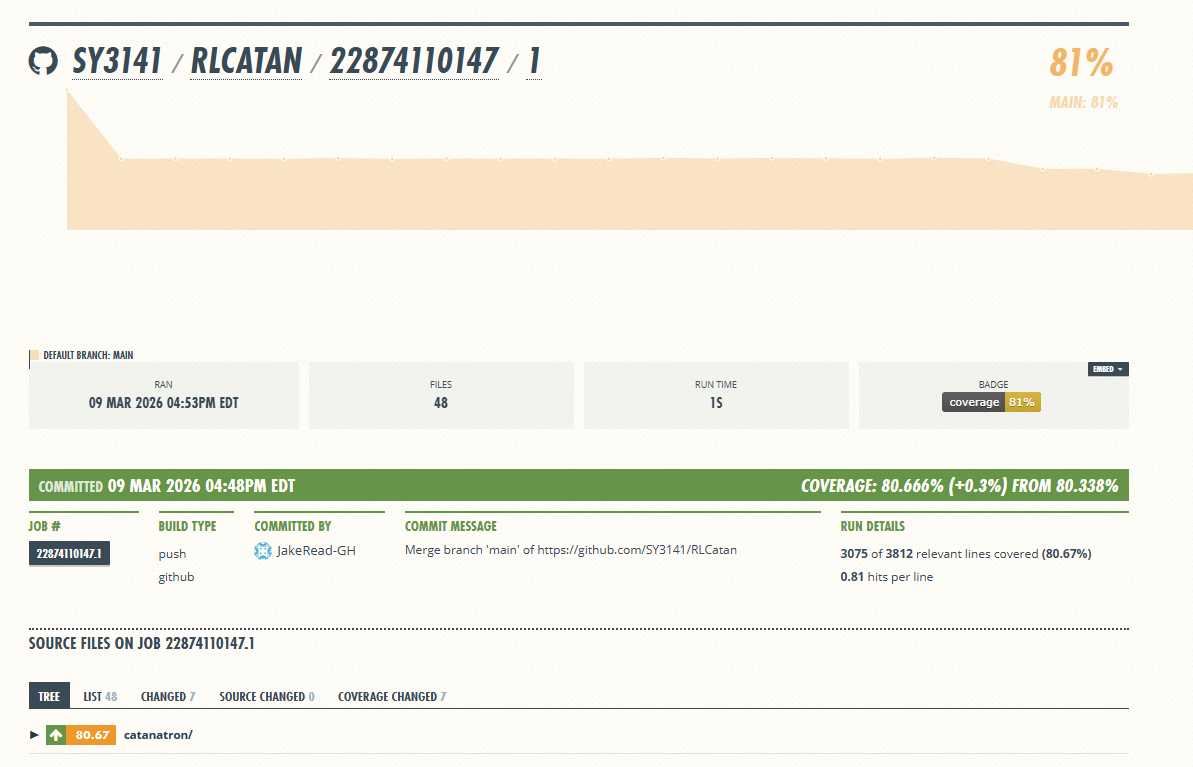
\includegraphics[width=0.8\textwidth]{coveralls_report}
    \caption{Coveralls Code Coverage Report}
\end{figure}

\newpage{}
\section*{Appendix --- Reflection}

The information in this section will be used to evaluate the team members on the
graduate attribute of Reflection.

\input{../Reflection.tex}

\begin{enumerate}
  \item What went well while writing this deliverable? 
  \item What pain points did you experience during this deliverable, and how
    did you resolve them?
  \item Which parts of this document stemmed from speaking to your client(s) or
  a proxy (e.g. your peers)? Which ones were not, and why?
  \item In what ways was the Verification and Validation (VnV) Plan different
  from the activities that were actually conducted for VnV?  If there were
  differences, what changes required the modification in the plan?  Why did
  these changes occur?  Would you be able to anticipate these changes in future
  projects?  If there weren't any differences, how was your team able to clearly
  predict a feasible amount of effort and the right tasks needed to build the
  evidence that demonstrates the required quality?  (It is expected that most
  teams will have had to deviate from their original VnV Plan.)
  \item Reflect on your use of CI for continuous integration testing (regression
  testing). Did your CI work to gatekeep your PRs?  Would it have been helpful
  if you got your CI working earlier in the project?  What are your plans to use
  CI for testing in future projects?
\end{enumerate}
    
\subsection{Answers}
For this reflection, we decided all of the questions were better answered as one cohesive reflection rather than answering each question individually.
    \begin{enumerate}
        \item We would say that overall this deliverable went quite smoothly.
        It certainly felt like less of a time crunch than previous documents, such as the SRS.
        This was mostly because we created a solid original VnV plan, so carrying it out did not present many major hurdles.
        As we will mention in a later answer, we had to make some minor modifications to certain planned tests, but for the most part, they were executed very closely to how they were originally written.
        \item
        The main pain point was recruiting participants for the usability study. Because Catan has a steep learning curve, we needed testers who already understood the game to provide meaningful feedback. Finding enough qualified users was challenging. We resolved this by reaching out to student groups and personal networks to recruit seven participants, which allowed us to complete the usability evaluation despite a tighter schedule.  
        Another significant challenge was the shift away from the original Computer Vision (CV)
        system. The technical complexity of real-time board detection proved to be too resource-intensive
        We resolved this by pivoting to a browser-based bot that users could play against or watch,
        which kept the focus on learning and gameplay rather than CV hardware issues.
        \item
        Several decisions in this deliverable were guided by client and proxy feedback.
        The suggestion of an LLM-based explanation system came from our supervisor, who
        suggested a tool that could explain its reasoning in natural language after hearing about our usability issues.
        Usability insights were collected from a proxy group of peers and acquaintances familiar with Catan, 
        helping us refine interface clarity, navigation, and tooltip visibility. 
        Other decisions, including removing the CV module and shifting from an AI recommendation
        engine to a playable learning bot, were internal pivots to make the system more practical and 
        accessible in a browser environment.
        \item
        The Verification and Validation activities deviated from the original plan due to these
        shifts in scope and architecture. Initial plans emphasized CV accuracy and board 
        reconstruction, but these were replaced with evaluations of UI responsiveness and AI logic 
        transparency. We also transitioned from testing recommendation accuracy to assessing the 
        educational value and gameplay flow of the bot. Furthermore, many planned requirement 
        tests were written before the final codebase structure was known, making some tests 
        redundant or infeasible. In future projects, we would treat the VnV Plan as a living document, 
        updating it alongside code development to better anticipate architectural changes and evolving project goals.
      \item CI/CD was a critical part of our development process.
        It was actually one of the first things we set up when we started the project, since our project integrates with the Catanatron simulator.
        It was essential to have automated testing in place to ensure that new code didn’t break existing functionality.
        We also set up linting and coveralls for coverage reports on each commit at that time, which has helped us maintain code quality and came in handy for the coverage section of this report.
        We always checked for passing tests before merging any PRs, and on a couple occasions that helped catch some regressions and integration issues before they became a problem.
        I'll be sticking to this approach for future projects, as it's been a great help keeping the codebase in order.
        After working with SonarQube in this report, I'm also considering adding that to the pipeline for future projects as well, to get more info on quality over time rather than the single snapshot we took here.
      \end{enumerate}
    

\end{document}